\section{La regla de aprendizaje y funciones de error}

Entonces tomando como base el perceptrón, una vez obtenidas las salidas con una primera iteración nos daremos cuenta que tan lejos o que tan cerca estuvimos de la respuesta correcta, con esto darnos la oportunidad de que pesos ajustar respecto a sus entradas, en la segunda iteración. Ahora para facilitarnos esto y tomando en cuenta que el entrenamiento consiste en varias iteraciones hasta llegar a aprender la tarea T, hacemos uso de una función de error que nos ayude a minimizar la diferencia de error en las salidas. Esto también es conocido como la regla de aprendizaje, para cada neurona en la capa de salida se le calcula la desviación a la función objetivo, denotado como $\delta$. El cual utilizamos para cambiar los pesos del perceptrón (ver fig \ref{fig:errorP}). 

\begin{figure}[h]
 \centering
 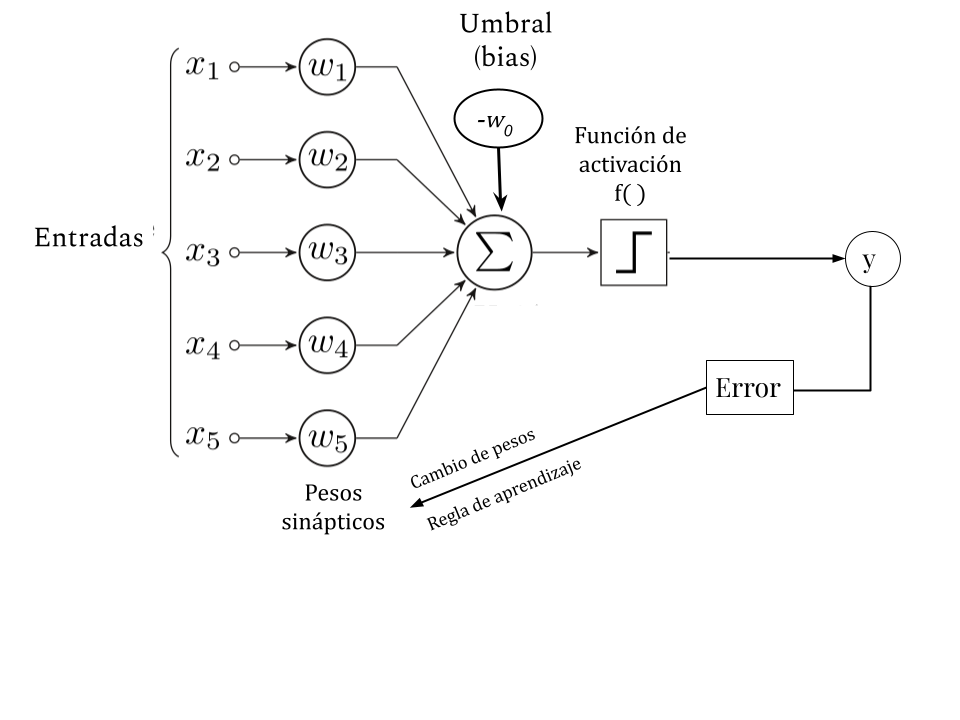
\includegraphics[scale=0.5]{../Figuras/ErrorPerceptron.png}
 \caption{Modelo estandar de un perceptrón.}
 \label{fig:errorP}
\end{figure}

Usualmente el principio del entrenamiento se asignan pesos aleatorios, a medida que avance el entrenamiento se van modificando con cada iteración, así \(w_{i} \leftarrow w_{i} + \Delta w_{i}\). Esto con base a \emph{la regla de aprendizaje} donde: 

\begin{equation}
 \Delta w_{i} = \eta(t - o)x_{i}
\end{equation}

 
Con $t$ la salida deseada, $o$ la salida generada, $\eta$ la taza de aprendizaje (learning rate) y $x_{i}$ la entrada. Lo que hace la taza de aprendizaje es moderar el rango que los pesos son cambiados con cada iteración. Normalmente se toman valores muy pequeños y conforme se logran ajustar los pesos se minimiza aun más.

Ahora supon que logramos que el perceptrón aprenda los datos de entrada, esto nos indica que $t = o$, haciendo que \(\Delta w_{i} = 0\), por tanto ningun peso se actualice. En nuestra etapa de validación, en un ejemplar los da la salida $y = -1$, cuando lo idicado es $1$. Entonces seguido de esa prueba necesitamos hacer cambio de la taza de aprendizaje para volver a ajustar los pesos correctamente.

Para entrenar un perceptrón, utilizamos cualquier método de optimización de funciones para encontrar los parámetros $w$ que minimizan el error con alguna de las siguientes funciones de error:

\begin{description}
 \item \textbf{Hebbian}, asume que si dos neuronas vecinas se activan y desactivan al mismo tiempo, los pesos que conectan estas neuranas deberian aumentar (los valores de entrada incrementan), si no hay correlación entre neuronas sus pesos no deberían cambiar, si una neurona se desactiva cuando la neurona presinaptica manda sus entradas, los pesos que las conectan deben disminuir. El inicio los pesos empiezan en cero $w_{n} = 0$, esta regla se usa en modelos de aprendizaje no supervisado. \[w_{ij} = w_{ij} * x_{j} * y_{i}\]   
 \item \textbf{Diferencias al cuadrado}, también conocida como regla del perceptrón, es la suma de cuadrados de errores que se tuvieron con cada ejemplar el el conjunto de entranamiento. Los podemos decribir como: 
 
 \begin{equation}
   \dfrac{1}{2m}\sum{m=0}^{M-1} (y_{m} - a_{m})^2
 \end{equation}
 
 con $y_{m} y a{m}$, la salida obtenida dado un ejemplar $m$ y la salida correcta del ejemplar $m$ respectivamente.
 \item \textbf{Entropía cruzada.} Se usa para problemas de clasificación ya que su comportamiento es más suave (soft) y permite hacer clasificaciones más certeras. Se define como:

 \begin{equation}
  L (\Theta) = -\dfrac{1}{m}\sum{M-1}^{m=0}(y^(m)log(a_{m}) + (1-y_{m}) log(1-a_{m})) 
 \end{equation}

\end{description}
